%*****************************************
\chapter{Evaluation}
\label{ch:evaluation}
%*****************************************
%\hint{This chapter should describe how the evaluation of the implemented mechanism was done. \\ \\
%1. Which evaluation method is used and why? Simulations, prototype? \\
%2. What is the goal of the evaluation? Comparison? Proof of concept? \\
%3. Wich metrics are used for characterizing the performance, costs, fairness, and efficiency of the system?\\
%4. What are the parameter settings used in the evaluation and why? If possible always justify why a certain threshold has been chose for a particular parameter.  \\
%5. What is the outcome of the evaluation? \\ \\
%The section should have a length of about five to ten pages.}
The following chapter presents the results achieved throughout this thesis and aims to explain their evaluation. First, the intended goal of each experiment is stated, including a  formulation in terms of validatable benchmarks. Subsequently, the process which extracts legible data from the framework is developed. The visualized data follows, and finally, the results are analyzed.

\section{Reproduction}
\subsection*{Goal and Benchmarks}
As the latter sections evaluate explorative experiments, the validity of the framework which supports them is crucial. We trained the first two models described in sections [4] and [5] under the conditions J. Frankle and M. Corbin describe in their paper. The mismatch of weights previously described forms the only known difference.
J. Frankle and M. Corbin primarily report the accuracy achieved by their implementations at the epoch of a simple stopping criterion. They executed each experiment five times and plot the mean alongside the minimum and maximum, which are represented through error bars. Additionally, they reperformed the same experiments ten times, but applied the masks, found after each epoch, to randomly reinitialized networks. The results were visualized in the same manner. [cite LTH]
On the left side of [figure 6.1] and [figure 6.2], these measures are presented for the MNIST-FCN and the CIFAR10-CNN-6, respectively. Both plots are taken from the Lottery Ticket Hypothesis paper, but we cleaned up the latter one and brought it up to scale for improved legibility.[footnote]  The goal of this reproduction is to produce results within the reported confidence intervals of accuracy in the Lottery Ticket Hypothesis paper.  

\subsection*{Evaluation Setup}
As the produced framework does not provide any early stopping criterion, we display the full range of accuracy a given architecture achieves after convergence. A line visualizes the mean, while a gray band denotes the interval between maximal and minimal achieved accuracy. As a positive side-effect, this setup increases the breadth of visualized data in the following explorative experiments because it is parameter-agnostic concerning the early stopping criterion. Finally,  as J. Frankle and M. Corbin present training accuracies for the MNIST-Lenet-FCN architecture, we visualize the same measure for additional points of comparison.\footnote{
	For the Conv6 architecture, the effective pruning rate per iteration amalgamate its dense and convolutional pruning rate. We remind that the disagreement in the number of weights in the dense layers between our framework and the Lottery Ticket Hypothesis paper also results in a different pruning rate per epoch. 
} 
\subsection*{Evaluation Results}
As seen in figure [6.1], the MNIST-Lenet-FCN implementation we provide achieves a lower accuracy than reported by J. Frankle and M. Corbin. Additionally, it does not show an interim improvement and degrades significantly faster at advanced pruning iterations. Said degradation is qualitatively similar to the behavior of the randomly reinitialized networks.
The comparison in figure [6.2] yields similar results. While the CIFAR10-CNN-6 implementation produces the same accuracy as a full network, it degrades as quickly as J. Frankel and M. Corbin's reinitialized networks. Most of its graph falls into the deviation intervals they visualized.

\begin{figure}
	\begin{minipage}{\textwidth}
		\centering
		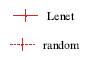
\includegraphics[width=100px]{gfx/7-Evaluation/LTH_3_legend.png}
	\end{minipage}
	\begin{minipage}{0.5\textwidth}
		\centering
		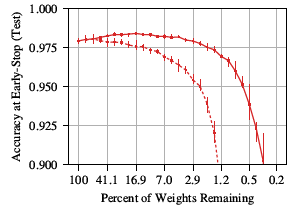
\includegraphics[height=180px]{gfx/7-Evaluation/LTH_0.png}
		\caption*{LTH-paper: Accuracy after convergence}
		\label{?}
	\end{minipage}\hfill
	\begin{minipage}{0.5\textwidth}
		\centering
		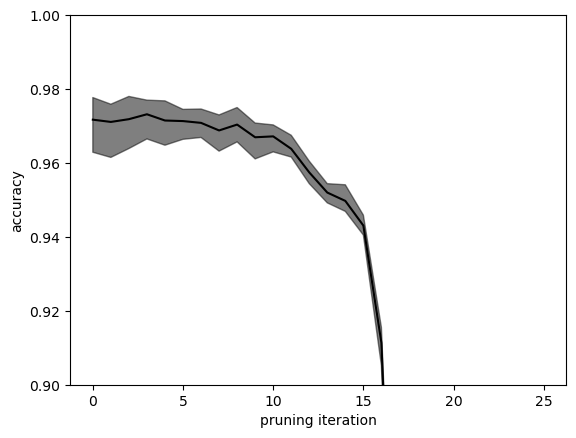
\includegraphics[height=170px]{gfx/Experiments/Reproduction-MNIST-FCN/accuracy/converged.png}
		\caption*{Thesis-Framework: Accuracy after convergence}
		\label{?}
	\end{minipage}
\end{figure}

\begin{figure}
	\begin{minipage}{\textwidth}
		\centering
		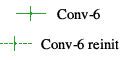
\includegraphics[width=100px]{gfx/7-Evaluation/LTH_4_legend.png}
	\end{minipage}
	\begin{minipage}{0.5\textwidth}
		\centering
		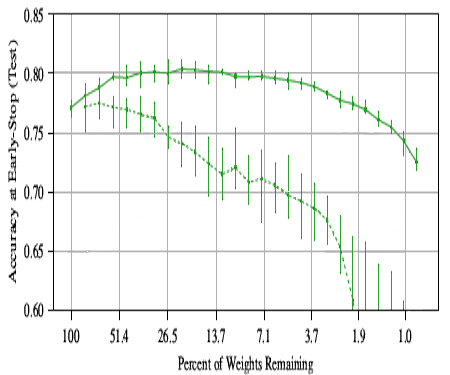
\includegraphics[height=175px]{gfx/7-Evaluation/LTH_CNN_clean.png}
		\caption*{LTH-paper: Accuracy after convergence}
		\label{?}
	\end{minipage}\hfill
	\begin{minipage}{0.5\textwidth}
		\centering
		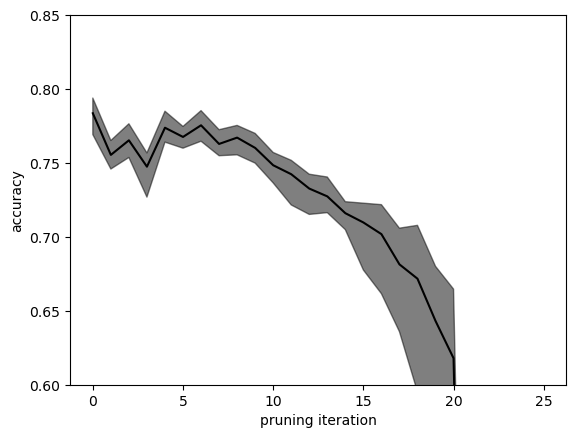
\includegraphics[height=175px]{gfx/Experiments/Reproduction-CIFAR10-CNN/accuracy/LTH.png}
		\caption*{Thesis-Framework: Accuracy after convergence}
		\label{?}
	\end{minipage}
\end{figure}

\begin{figure}
	\begin{minipage}{\textwidth}
		\centering
		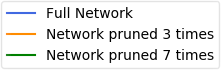
\includegraphics[width=100px]{gfx/7-Evaluation/LTH_1_legend.png}
	\end{minipage}
	\begin{minipage}{0.5\textwidth}
		\centering
		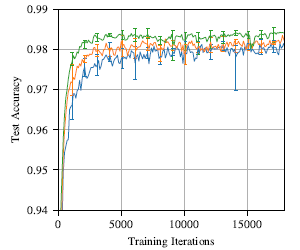
\includegraphics[height=175px]{gfx/7-Evaluation/LTH_1.png}
		\caption*{LTH-paper: pruned 0|3|7 times}
		\label{?}
	\end{minipage}\hfill
	\begin{minipage}{0.5\textwidth}
		\centering
		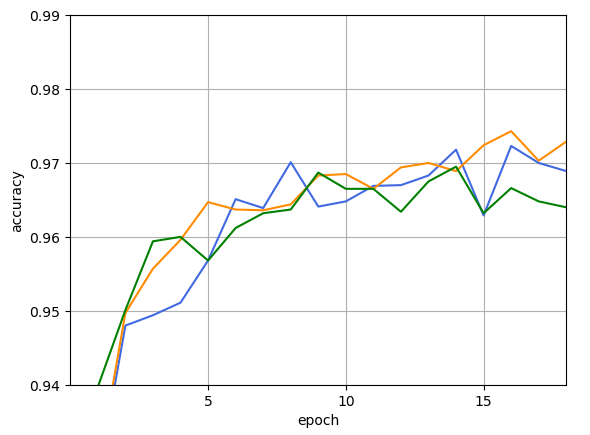
\includegraphics[height=175px]{gfx/Experiments/Reproduction-MNIST-FCN/accuracy/LTH_1.png}
		\caption*{Thesis-Framework: pruned 0|3|7 times}
		\label{?}
	\end{minipage}
\end{figure}

\begin{figure}
	\begin{minipage}{\textwidth}
		\centering
		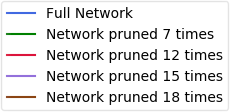
\includegraphics[width=100px]{gfx/7-Evaluation/LTH_2_legend.png}
	\end{minipage}
	\begin{minipage}{0.5\textwidth}
		\centering
		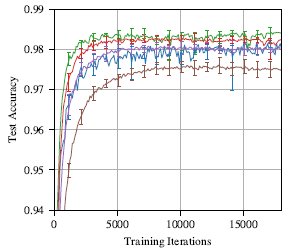
\includegraphics[height=175px]{gfx/7-Evaluation/LTH_2.png}
		\caption*{LTH-paper: pruned 0|7|12|15|18 times}
		\label{?}
	\end{minipage}\hfill
	\begin{minipage}{0.5\textwidth}
		\centering
		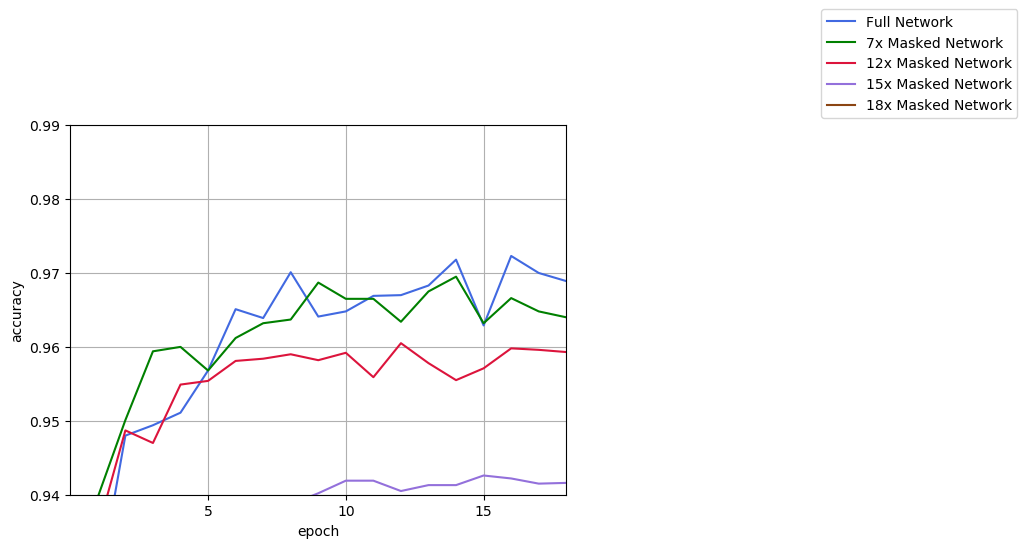
\includegraphics[height=175px]{gfx/Experiments/Reproduction-MNIST-FCN/accuracy/LTH_2.png}
		\caption*{Thesis-Framework: pruned 0|7|12|15|18 times}
		\label{?}
	\end{minipage}
\end{figure}
\subsection*{Analysis of Results}
The implementations of the provided framework do not reproduce the results presented in the Lottery Ticket Hypothesis paper, meaning that the framework is not validated. This poses the question of how to proceed with the remaining experiments, which we discuss in the corresponding "Goal and Benchmarks" subsections.
While the framework did not fulfill the primary goal of the experiment, two phenomena remain unclear and intriguing:
The MNIST-Lenet-FCN architecture produces through our implementation of the Lottery Ticket algorithm degrades only by one percentage point under compression of up to ten times. Such a result is comparable to various pruning methods discussed in chapter [3]. 

%*****************************************

\section{Transfer}
\subsection*{Goal and Benchmarks}
While the reproduction experiments did not validate the framework, it still pruned the MNIST-Lenet-FCN to a degree comparable to contemporary work through, and it did so through the masking of networks with frozen initialization. As such, the transfer to another field still might yield another pruning tool for additional tasks and applications. If the framework prunes about 90 percent of weight without the sacrifice of prediction quality, we consider the transfer succesful.
\subsection*{Evaluation Setup}
While figure [6.3] presents the accuracies collected in the same manner as before, fewer pruning iterations are displayed. Due to the sheer size of the 20Newsgroups-End2End architecture and the way our framework interacts with TensorFlow 2.0 to produce pruned networks severely limited the number of pruning iterations, a single experiment could afford to run without overflowing the memory of our computing devices. We managed to run experiments with ten pruning iterations, the minimal number to prune a network to a competitive degree.
\subsection*{Evaluation Results}
The right side of figure [6.4] shows that the 20Newsgroups-End2End architecture retains its accuracy even if about 90 percent of its weights are pruned. Additionally, the networks of the intermediate pruning epochs show an accuracy improvement of at least one percentage point.
\begin{figure}
	\begin{minipage}{0.5\textwidth}
		\centering
		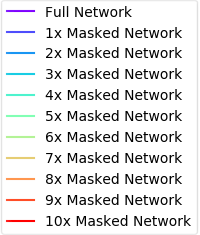
\includegraphics[width=100px]{gfx/7-Evaluation/20Newsgroups_legend.png}
	\end{minipage}
	\begin{minipage}{0.5\textwidth}
		\centering
		%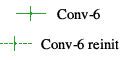
\includegraphics[width=100px]{gfx/7-Evaluation/LTH_4_legend.png}
	\end{minipage}
	\\
	\begin{minipage}{0.5\textwidth}
		\centering
		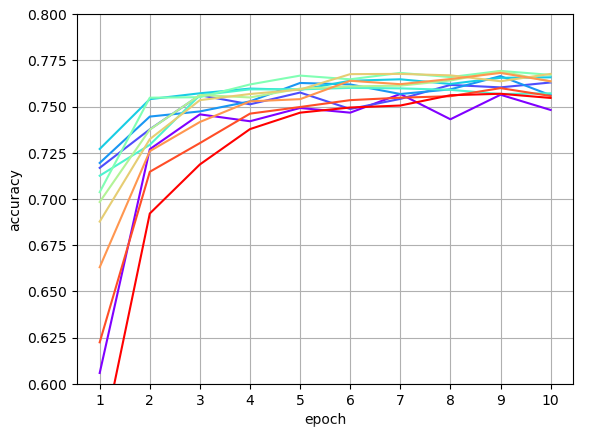
\includegraphics[height=175px]{gfx/Experiments/Transfer-20Newsgroups-CNN/accuracy/10_iterations.png}
		\caption*{Accuracy on 20Newsgroups pruned 0-10 times}
		\label{fig:CIFAR10accuracy15}
	\end{minipage}\hfill
	\begin{minipage}{0.5\textwidth}
		\centering
		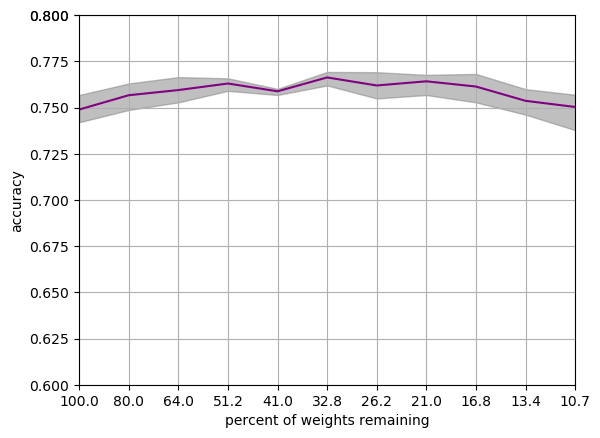
\includegraphics[height=175px]{gfx/Experiments/Transfer-20Newsgroups-CNN/accuracy/converged.png}
		\caption*{Accuracy on 20Newsgroups after convergence}
		\label{?}
	\end{minipage}
\end{figure}

\subsection*{Analysis of Results}
According to the previously defined goal, the transfer was successful, which shows that non-image-recognition architectures can contain efficient subnetworks upon initialization.

%*****************************************

\section{Early Tickets}
\subsection*{Goal and Benchmarks}
\subsection*{Evaluation Setup}
\subsection*{Evaluation Results}
\begin{figure}
	\begin{minipage}{\textwidth}
		\centering
		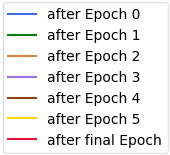
\includegraphics[width=100px]{gfx/7-Evaluation/LTH_5_legend.png}
	\end{minipage}
	\begin{minipage}{0.5\textwidth}
		\centering
		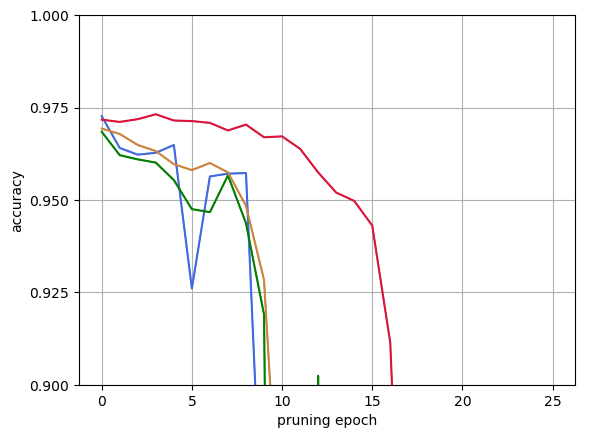
\includegraphics[height=175px]{gfx/Experiments/EarlyTicket-MNIST-FCN/012.png}
		\caption*{Ticket candidates pruned at epochs 0|1|2}
		\label{?}
	\end{minipage}\hfill
	\begin{minipage}{0.5\textwidth}
		\centering
		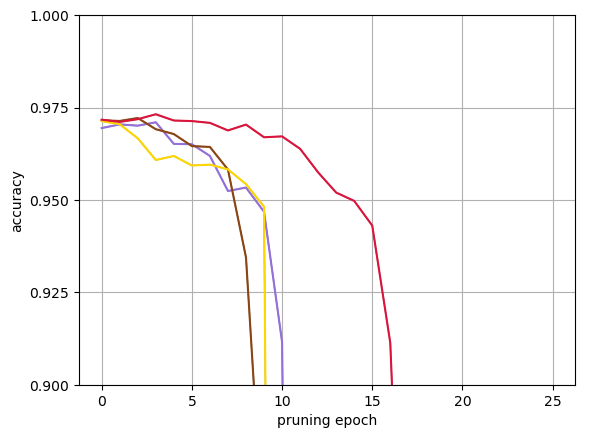
\includegraphics[height=175px]{gfx/Experiments/EarlyTicket-MNIST-FCN/345.png}
		\caption*{Ticket candidates pruned at epochs 3|4|5}
		\label{?}
	\end{minipage}
\end{figure}
\begin{figure}
	\begin{minipage}{\textwidth}
		\centering
		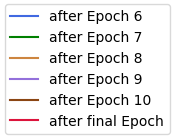
\includegraphics[width=100px]{gfx/7-Evaluation/LTH_6_legend.png}
	\end{minipage}
	\begin{minipage}{0.5\textwidth}
		\centering
		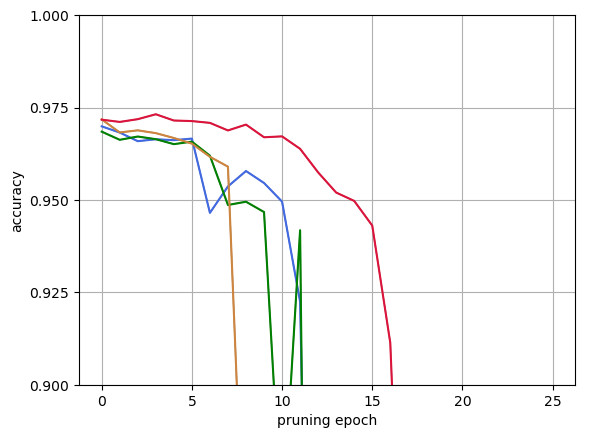
\includegraphics[height=175px]{gfx/Experiments/EarlyTicket-MNIST-FCN/678.png}
		\caption*{Ticket candidates pruned at epochs 6|7|8}
		\label{?}
	\end{minipage}\hfill
	\begin{minipage}{0.5\textwidth}
		\centering
		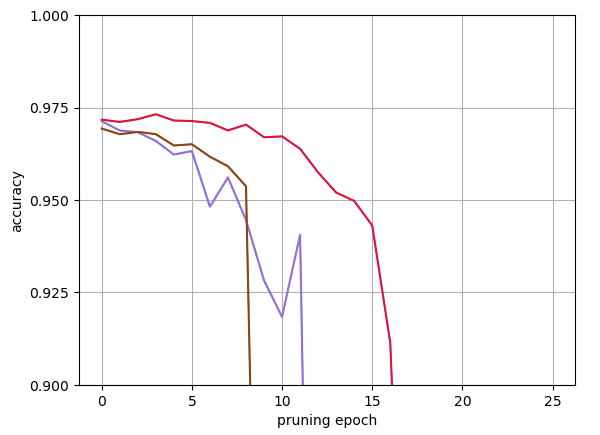
\includegraphics[height=175px]{gfx/Experiments/EarlyTicket-MNIST-FCN/910.png}
		\caption*{Ticket candidates pruned at epochs 9 and 10}
		\label{?}
	\end{minipage}
\end{figure}
\subsection*{Analysis of Results}
